\chapter{Технологический раздел}
\label{cha:impl}
В данном разделе представлены средства разработки программного
обеспечения, его тестирования, детали реализации и графический интерфейс приложения.

\section{Средства реализации}

Основным средством разработки является язык программирования. Был выбран язык программирования C++. Данный выбор обоснован высокой скоростью работы языка, поддержкой объектно-ориентированного подхода программирования и строгой типизаций \cite{cpplang}. 

В связи с гибкой архитектурой приложения возможна быстрая интеграция любой библиотеки графического интерфейса (GUI). Было принято решение использовать Qt Framework, который предоставляет большой набор базовых компонентов и поддерживает платформы Linux, Windows, macOS и другие \cite{qt_widgets}. 

Для поддержания качества кода было принято использовать инструменты статического анализа кода cpplint\cite{cpplint} и cppcheck\cite{cppcheck}, отладчик использования памяти valgrind\cite{valgrind}. 

Для тестирование приложения предлагается к использованию библиотека модульного тестирования Google Test, которая имеет широкий функционал для написания тестов, конфигурации объектов и подмены сущностей во время тестирования \cite{googletest}.

\section{Детали реализации алгоритмов}

\lstinputlisting[language=c,caption={Отрисовка полигона с помощью Z-буфера},label=lst:sample01]{code/polygon.cpp}
\lstinputlisting[language=c,caption={Формирования списка ребер},label=lst:sample02]{code/makeedges.cpp}

\section{Графический интерфейс}

Был разработан графический интерфейс приложения. Он представлен на рисунке \ref{fig:gui_window}. 

\begin{figure}[h!]
    \centering
    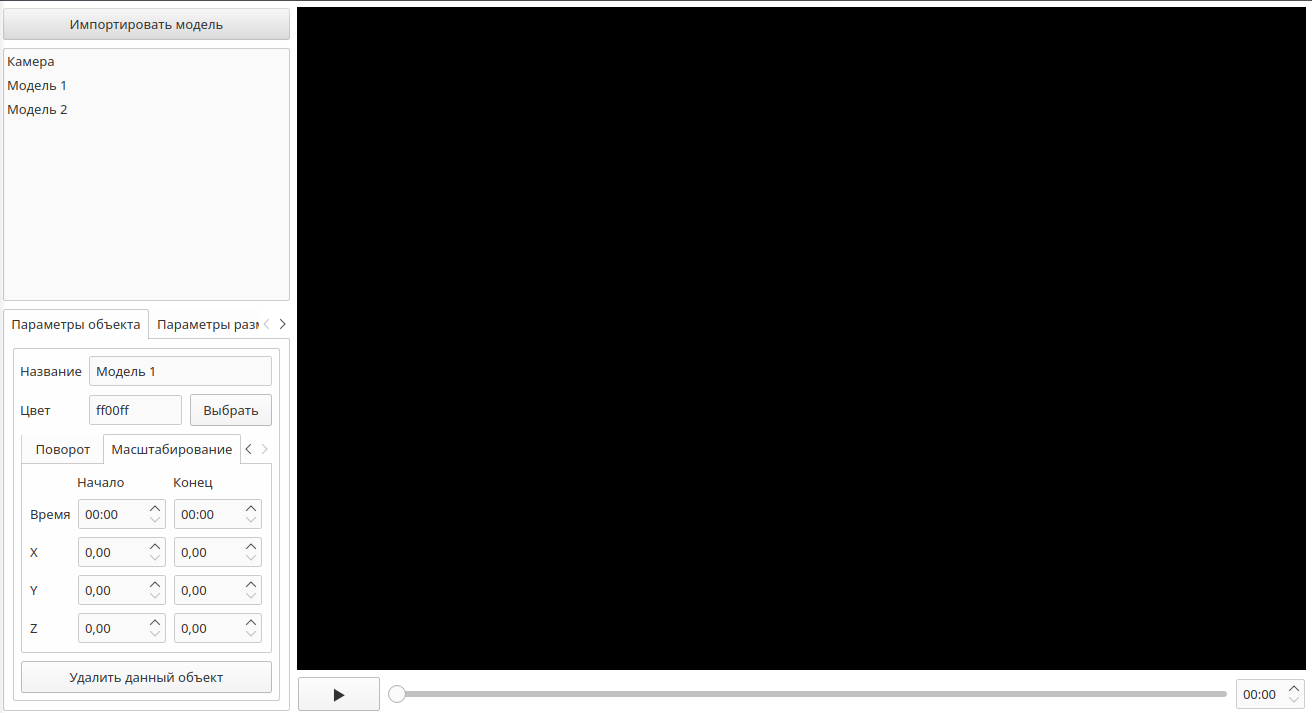
\includegraphics[width=0.9\columnwidth]{img/gui/common.png}
    \caption{Общий вид окна}
    \label{fig:gui_window}
\end{figure}

В правой половине окна расположены предпросмотр сцены и временная шкала. В левой половине список объектов сцены и параметры в виде вкладок. Все вкладки параметров представлены на рисунке \ref{fig:gui_tabs}

\begin{figure}[h!]
    \centering
    \begin{minipage}[h]{0.32\linewidth}
        \center{
            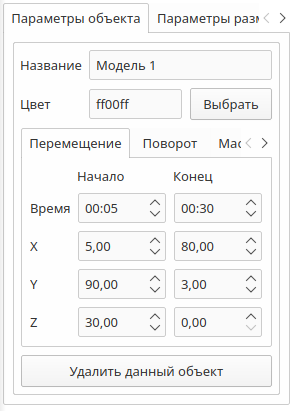
\includegraphics[width=\linewidth]{img/gui/tab1.png} \\ а)
            }
    \end{minipage}
    \hfill\begin{minipage}[h]{0.32\linewidth}
        \center{
            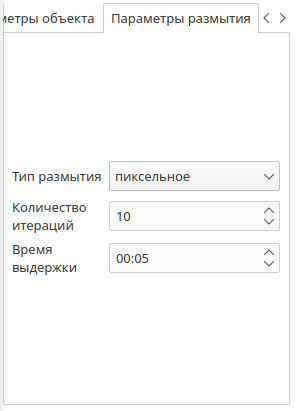
\includegraphics[width=\linewidth]{img/gui/tab2.png} \\ б)
            }
    \end{minipage}
    \hfill
    \begin{minipage}[h]{0.32\linewidth}
        \center{
            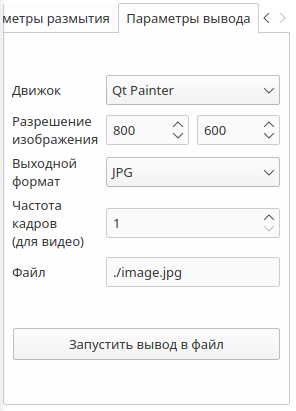
\includegraphics[width=\linewidth]{img/gui/tab3.png} \\ в)
            }
    \end{minipage}
    \caption{Вкладка параметров \\
    а) сцены объекта 
    б) размытия движения
    в) вывода в файл}
    \label{fig:gui_tabs}
\end{figure}

Для изменения параметров определенного объекта пользователю необходимо выбрать нужный объект из списка объектов и внести изменения во вкладке параметров объекта. Также возможно внести изменения в параметры размытия и вывода. 

\section{Вывод}

В данном разделе были описаны средства разработки программного
обеспечения, его тестирования, детали реализации и графический интерфейс приложения.



% В данном разделе описано изготовление и требование всячины. Кстати,
% в Latex нужно эскейпить подчёркивание (писать <<\verb|some\_function|>> для \Code{some\_function}).

% \ifPDFTeX
% Для вставки кода есть пакет \Code{listings}. К сожалению, пакет \Code{listings} всё ещё
% работает криво при появлении в листинге русских букв и кодировке исходников utf-8.
% В данном примере он (увы) на лету конвертируется в koi-8 в ходе сборки pdf.

% Есть альтернатива \Code{listingsutf8}, однако она работает лишь с
% \Code{\textbackslash{}lstinputlisting}, но не с окружением \Code{\textbackslash{}lstlisting}

% Вот так можно вставлять псевдокод (питоноподобный язык определен в \Code{listings.inc.tex}):

% \begin{lstlisting}[style=pseudocode,caption={Алгоритм оценки дипломных работ}]
% def EvaluateDiplomas():
%     for each student in Masters:
%         student.Mark := 5
%     for each student in Engineers:
%         if Good(student):
%             student.Mark := 5
%         else:
%             student.Mark := 4
% \end{lstlisting}

% Еще в шаблоне определен псевдоязык для BNF:

% \begin{lstlisting}[style=grammar,basicstyle=\small,caption={Грамматика}]
%   ifstmt -> "if" "(" expression ")" stmt |
%             "if" "(" expression ")" stmt1 "else" stmt2
%   number -> digit digit*
% \end{lstlisting}

% В листинге~\ref{lst:sample01} работают русские буквы. Сильная магия. Однако, работает
% только во включаемых файлах, прямо в \TeX{} нельзя.

% % Обратите внимание, что включается не ../src/..., а inc/src/...
% % В Makefile есть соответствующее правило для inc/src/*,
% % которое копирует исходные файлы из ../src и конвертирует из UTF-8 в KOI8-R.
% % Кстати, поэтому использовать можно только русские буквы и ASCII,
% % весь остальной UTF-8 вроде CJK и египетских иероглифов -- нельзя.

% \lstinputlisting[language=C,caption=Пример (\Code{test.c}),label=lst:sample01]{inc/src/test.c}

% \else

% Для вставки кода есть пакет \texttt{minted}. Он хорош всем кроме: необходимости Python (есть во всех нормальных (нет, Windows, я не про тебя) ОС) и Pygments и того, что нормально работает лишь в \XeLaTeX.

% \ifdefined\NoMinted
% Но к сожалению, у вас, по-видимому, не установлен Python или pygmentize.
% \else
% Можно пользоваться расширенным BFN:

% \begin{listing}[H]
% \begin{ebnfcode}
%  letter = "A" | "B" | "C" | "D" | "E" | "F" | "G"
%        | "H" | "I" | "J" | "K" | "L" | "M" | "N"
%        | "O" | "P" | "Q" | "R" | "S" | "T" | "U"
%        | "V" | "W" | "X" | "Y" | "Z" ;
% digit = "0" | "1" | "2" | "3" | "4" | "5" | "6" | "7" | "8" | "9" ;
% symbol = "[" | "]" | "{" | "}" | "(" | ")" | "<" | ">"
%        | "'" | '"' | "=" | "|" | "." | "," | ";" ;
% character = letter | digit | symbol | "_" ;
 
% identifier = letter , { letter | digit | "_" } ;
% terminal = "'" , character , { character } , "'" 
%          | '"' , character , { character } , '"' ;
 
% lhs = identifier ;
% rhs = identifier
%      | terminal
%      | "[" , rhs , "]"
%      | "{" , rhs , "}"
%      | "(" , rhs , ")"
%      | rhs , "|" , rhs
%      | rhs , "," , rhs ;
 
% rule = lhs , "=" , rhs , ";" ;
% grammar = { rule } ;
% \end{ebnfcode}
% \caption{EBNF определённый через EBNF}
% \label{lst:ebnf}
% \end{listing}

% А вот в листинге \ref{lst:c} на языке C работают русские комменты. Спасибо Pygments и Minted за это.

% \begin{listing}[H]
% \cfile{inc/src/test.c}
% \caption{Пример — test.c} 
% \end{listing}
% \label{lst:c}

% \fi
% \fi
% % Для вставки реального кода лучше использовать \texttt{\textbackslash lstinputlisting} (который понимает
% % UTF8) и стили \Code{realcode} либо \Code{simplecode} (в зависимости от размера куска).




% Можно также использовать окружение \Code{verbatim}, если \Code{listings} чем-то не
% устраивает. Только следует помнить, что табы в нём <<съедаются>>. Существует так же команда \Code{\textbackslash{}verbatiminput} для вставки файла.

% \begin{verbatim}
% a_b = a + b; // русский комментарий
% if (a_b > 0)
%     a_b = 0;
% \end{verbatim}

%%% Local Variables:
%%% mode: latex
%%% TeX-master: "rpz"
%%% End:
